\hypertarget{contributions}{%
\section{Contributions}\label{contributions}}

The material in this chapter expands on work presented in

\textbf{Insert citation of amorphous Kitaev paper here}

which was a joint project of the first three authors with advice and guidance from Willian and Johannes. The project grew out of an interest Gino, Peru and I had in studying amorphous systems, coupled with Johannes' expertise on the Kitaev model. The idea to use voronoi partitions came from \autocite{marsalTopologicalWeaireThorpe2020} and Gino did the implementation of this. The idea and implementation of the edge colouring using SAT solvers, the mapping from flux sector to bond sector using A* search were both entirely my work. Peru came up with the ground state conjecture and implemented the local markers. Gino and I did much of the rest of the programming for Koala while pair programming and 'whiteboard'ing, this included the phase diagram, edge mode and finite temperature analyses as well as the derivation of the projector in the amorphous case.

\hypertarget{introduction}{%
\section{Introduction}\label{introduction}}

\hypertarget{fig:intro_figure_by_hand}{%
\begin{figure}
\centering
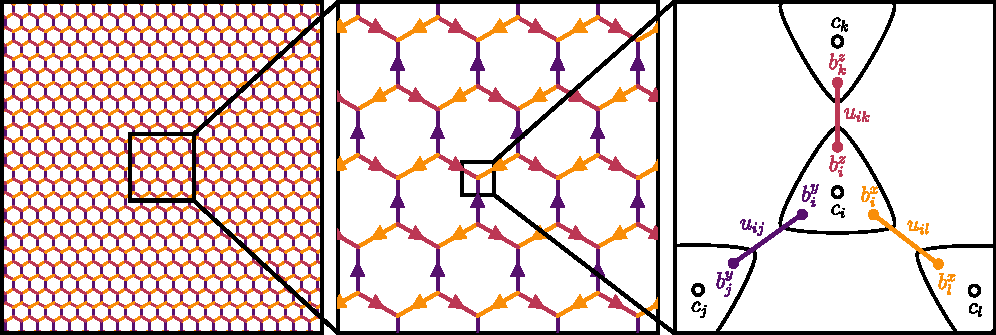
\includegraphics[width=1\textwidth,height=\textheight]{figure_code/amk_chapter/intro/honeycomb_zoom/intro_figure_by_hand}
\caption[{The Kitaev Honeycomb Model}]{\textbf{(a)} The standard Kitaev model is defined on a honeycomb lattice. The special feature of the honeycomb lattice that makes the model solvable is that each vertex is joined by exactly three bonds, i.e.~the lattice is trivalent. One of three labels is assigned to each \textbf{(b)}. We represent the antisymmetric gauge degree of freedom \(u_{jk} = \pm 1\) with arrows that point in the direction \(u_{jk} = +1\) \textbf{(c)}. The Majorana transformation can be visualised as breaking each spin into four Majoranas which then pair along the bonds. The pairs of x,y and z Majoranas become part of the classical \(\mathbb{Z}_2\) gauge field \(u_{ij}\). This leavies a single Majorana \(c_i\) per site.}
\label{fig:intro_figure_by_hand}
\end{figure}
}

The Kitaev Honeycomb model \[H =  - \sum_{\langle j,k\rangle_\alpha} J^{\alpha}\sigma_j^{\alpha}\sigma_k^{\alpha},\] is remarkable because it combines three key properties.

First, the form of the Hamiltonian plausibly be realised by a real material. Candidate materials, such as \(\alpha\mathrm{-RuCl}_3\), are known to have sufficiently strong spin-orbit coupling and the correct lattice structure to behave according to the Kitaev Honeycomb model with small corrections \autocite{banerjeeProximateKitaevQuantum2016,trebstKitaevMaterials2022}.

\textbf{expand later: Why do we need spin orbit coupling and what will the corrections be?}

Second, its ground state is the canonical example of the long sought after quantum spin liquid state. Its excitations are anyons, particles that can only exist in two dimensions that break the normal fermion/boson dichotomy. Anyons have been the subject of much attention because, among other reasons, they can be braided through spacetime to achieve noise tolerant quantum computations \autocite{freedmanTopologicalQuantumComputation2003}.

Third, and perhaps most importantly, this model is a rare many body interacting quantum system that can be treated analytically. It is exactly solvable. We can explicitly write down its many body ground states in terms of single particle states \autocite{kitaevAnyonsExactlySolved2006}. The solubility of the Kitaev Honeycomb Model, like the Falikov-Kimball model of chapter 1, comes about because the model has extensively many conserved degrees of freedom. These conserved quantities can be factored out as classical degrees of freedom, leaving behind a non-interacting quantum model that is easy to solve.

\hypertarget{amorphous-systems}{%
\subsection{Amorphous Systems}\label{amorphous-systems}}

\textbf{Insert discussion of why a generalisation to the amorphous case is interesting}

This chapter details the physics of the Kitaev model on amorphous lattices.

It starts by expanding on the physics of the Kitaev model. It will look at the gauge symmetries of the model as well as its solution via a transformation to a Majorana hamiltonian. This discussion shows that, for the the model to be solvable, it needs only be defined on a trivalent, tri-edge-colourable lattice \autocite{Nussinov2009}.

The methods section discusses how to generate such lattices and colour them. It also explain how to map back and forth between configurations of the gauge field and configurations of the gauge invariant quantities.

The results section begins by looking at the zero temperature physics. It presents numerical evidence that the ground state of the Kitaev model is given by a simple rule depending only on the number of sides of each plaquette. It assesses the gapless, Abelian and non-Abelian, phases that are present, characterising them by the presence of a gap and using local Chern markers. Next it looks at spontaneous chiral symmetry breaking and topological edge states. It also compares the zero temperature phase diagram to that of the Kitaev Honeycomb Model. Finally, we introduce flux disorder and demonstrate that there is a phase transition to a thermal metal state.

The discussion considers possible physical realisations of this model and the motivations for doing so. It also discusses how a well known quantum error correcting code defined on the Kitaev Honeycomb model could be generalised to the amorphous case.

\hypertarget{glossary}{%
\subsection{Glossary}\label{glossary}}

\begin{itemize}
\item
  Lattice: The underlying graph on which the models are defined. Composed of sites (vertices), bonds (edges) and plaquettes (faces).
\item
  The model : Used when I refer to properties of the the Kitaev model that do not depend on the particular lattice.
\item
  The Honeycomb model : The Kitaev Model defined on the honeycomb lattice.
\item
  The Amorphous model : The Kitaev Model defined on the amorphous lattices described here.
\end{itemize}

\textbf{The Spin Hamiltonian}

\begin{itemize}
\tightlist
\item
  Spin Bond Operators: \(\hat{k}_{ij} = \sigma_i^\alpha \sigma_j^\alpha\)
\item
  Loop Operators: \(\hat{W_p} = \prod_{<i,j>} k_{ij}\)
\item
  Plaquette Operators: Loops that enclose a single plaquette.
\end{itemize}

\textbf{The Majorana Model}

\begin{itemize}
\tightlist
\item
  Majorana Operators on site \(i\): \(\hat{b}^x_i, \hat{b}^y_i, \hat{b}^z_i, \hat{c}_i\)
\item
  Majorana Bond Operators: \(\hat{u}_{ij} = i \sigma_i^\alpha \sigma_j^\alpha\)
\item
  Loop Operators: \(\hat{W_p} = \prod_{<i,j>} u_{ij}\)
\item
  Plaquette Operators: Loops that enclose a single plaquette.
\item
  Gauge Operators: \(D_i = \hat{b}^x_i \hat{b}^y_i \hat{b}^z_i \hat{c}_i\)
\item
  The Extended Hilbert space: The larger Hilbert space spanned by the Majorana operators.
\item
  The physical subspace: The subspace of the extended Hilbert space that we identify with the Hilbert space of the original spin model.
\item
  The Projector \(\hat{P}\): The projector onto the physical subspace.
\end{itemize}

\textbf{Flux Sectors}

\begin{itemize}
\item
  Odd/Even Plaquettes: Plaquettes with an odd/even number of sides.
\item
  Fluxes \(\phi_i\): The expectation values of the plaquette operators \(\pm 1\) for even and \(\pm i\) for odd plaquettes.
\item
  Flux Sector: A subspace of Hilbert space in which the fluxes take particular values.
\item
  Ground state flux sector: The Flux Sector containing the lowest energy many body state.
\item
  Vortices: Flux excitations away from the ground state flux sector.
\item
  Dual Loops: A set of \(u_{jk}\) that correspond to loops on the dual lattice.
\item
  non-contractible loops or dual loops: The two loops topologically distinct loops on the torus that cannot be smoothly deformed to a point.
\item
  Topological Fluxes \(\Phi_{x}, \Phi_{y}\): The two fluxes associated with the two non-contractible loops.
\item
  Topological Transport Operators: \(\mathcal{T}_{x}, \mathcal{T}_{y}\): The two vortex-pair operations associated with the non-contractible \emph{dual} loops.
\end{itemize}

\textbf{Phases}

\begin{itemize}
\tightlist
\item
  The A phase: The three anisotropic regions of the phase diagram \(A_x, A_y, A_z\) where \(A_\alpha\) means \(J_\alpha >> J_\beta, J_\gamma\).
\item
  The B phase: The roughly isotropic region of the phase diagram.
\end{itemize}

\hypertarget{the-kitaev-model}{%
\subsection{The Kitaev Model}\label{the-kitaev-model}}

\hypertarget{commutation-relations}{%
\subsubsection{Commutation relations}\label{commutation-relations}}

Before diving into the Hamiltonian of the Kitaev model, the following describes the key commutation relations of spins, fermions and Majoranas.

\hypertarget{spins}{%
\paragraph{Spins}\label{spins}}

Skip this is you are familiar with the algebra of the Pauli matrices. Scalars like \(\delta_{ij}\) should be understood to be multiplied by an implicit identity \(\mathbb{1}\) where necessary.

We can represent a single spin\(-1/2\) particle using the Pauli matrices \((\sigma^x, \sigma^y, \sigma^z) = \vec{\sigma}\), these matrices all square to the identity \(\sigma^\alpha \sigma^\alpha = \mathbb{1}\) and obey nice commutation and exchange rules: \[\sigma^\alpha \sigma^\beta = \delta^{\alpha \beta} + i \epsilon^{\alpha \beta \gamma} \sigma^\gamma\] \[[\sigma^\alpha, \sigma^\beta] = 2 i \epsilon^{\alpha \beta \gamma} \sigma^\gamma\]

Adding site indices, spins at different spatial sites always commute \([\vec{\sigma}_i, \vec{\sigma}_j] = 0\) so when \(i \neq j\) \[\sigma_i^\alpha \sigma_j^\beta = \sigma_j^\alpha \sigma_i^\beta\] \[[\sigma_i^\alpha, \sigma_j^\beta] = 0\] while the previous equations hold for \(i = j\).

Two extra relations useful for the Kitaev model are the value of \(\sigma^\alpha \sigma^\beta \sigma^\gamma\) and \([\sigma^\alpha \sigma^\beta, \sigma^\gamma]\) when \(\alpha \neq \beta \neq \gamma\) these can be computed relatively easily by applying the above relations yielding: \[\sigma^\alpha \sigma^\beta \sigma^\gamma = i \epsilon^{\alpha\beta\gamma}\] and \[[\sigma^\alpha \sigma^\beta, \sigma^\gamma] = 0\]

\hypertarget{fermions-and-majoranas}{%
\paragraph{Fermions and Majoranas}\label{fermions-and-majoranas}}

The fermionic creation and anhilation operators are defined by the canonical anticommutation relations \[\begin{aligned}
\{f_i, f_j\} &= \{f^\dagger_i, f^\dagger_j\} = 0\\
\{f_i, f^\dagger_j\} &= \delta_{ij}
\end{aligned}\] which give us the exchange statistics and Pauli exclusion principle.

From fermionic operators, we can construct Majorana operators: \[\begin{aligned}
f_i         &= 1/2 (a_i + ib_i)\\
f^\dagger_i &= 1/2(a_i - ib_i)\\
a_i         &= f_i + f^\dagger_i = 2\Re f\\
b_i         &= 1/i(f_i - f^\dagger_i) = 2\Im f 
\end{aligned}\]

Majorana operators are the real and imaginary parts of the fermionic operators. Physically, they correspond to the orthogonal superpositions of the presence and absence of the fermion and are, thus, a kind of quasiparticle.

Once we involve multiple fermions, there is some freedom in how we can perform the transformation from \(n\) fermions \(f_i\) to \(2n\) Majoranas \(c_i\). The property that must be preserved, however, is that the Majoranas still anticommute:

\[ \{c_i, c_j\} = 2\delta_{ij}\]

\hypertarget{fig:visual_kitaev_1}{%
\begin{figure}
\centering
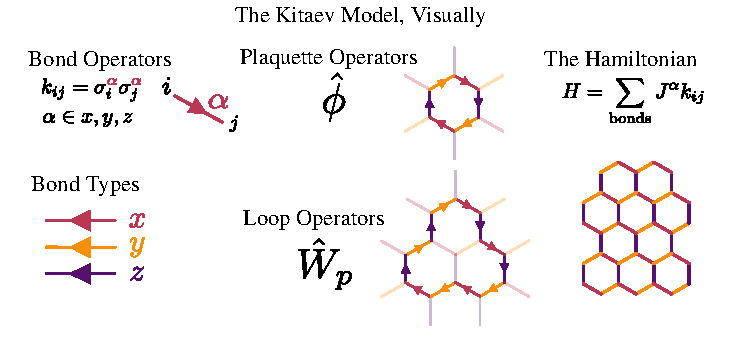
\includegraphics[width=1\textwidth,height=\textheight]{figure_code/amk_chapter/visual_kitaev_1}
\caption[{A Visual Intro to the Kitaev Model}]{A visual introduction to the Kitaev Model.}
\label{fig:visual_kitaev_1}
\end{figure}
}

\hypertarget{the-hamiltonian}{%
\subsubsection{The Hamiltonian}\label{the-hamiltonian}}

To start from the fundamentals, the Kitaev Honeycomb model is a model of interacting spin\(-1/2\)s on the vertices of a honeycomb lattice. Each bond in the lattice is assigned a label \(\alpha \in \{ x, y, z\}\) and that bond couples its two spin neighbours along the \(\alpha\) axis. See \cref{fig:visual_kitaev_1} for a diagram.

This gives us the Hamiltonian \[H =  - \sum_{\langle j,k\rangle_\alpha} J^{\alpha}\sigma_j^{\alpha}\sigma_k^{\alpha},\] where \(\sigma^\alpha_j\) is a Pauli matrix acting on site \(j\) and \(\langle j,k\rangle_\alpha\) is a pair of nearest-neighbour indices connected by an \(\alpha\)-bond with exchange coupling \(J^\alpha\) \autocite{kitaevAnyonsExactlySolved2006}. For notational brevity, it is useful to introduce the bond operators \(K_{ij} = \sigma_j^{\alpha}\sigma_k^{\alpha}\) where \(\alpha\) is a function of \(i,j\) that picks the correct bond type.

This Kitaev model has a set of conserved quantities that, in the spin language, take the form of Wilson loop operators \(W_p\) winding around a closed path on the lattice. The direction does not matter, but we will keep to clockwise here. We will use the term plaquette and the symbol \(\phi\) to refer to a Wilson loop operator that does not enclose any other sites, such as a single hexagon in a honeycomb lattice.

\[W_p = \prod_{\mathrm{i,j}\; \in\; p} K_{ij} = \sigma_1^z \sigma_2^x \sigma_2^y \sigma_3^y .. \sigma_n^y \sigma_n^y \sigma_1^z\]

\textbf{add a diagram of a single plaquette with labelled site and bond types}

In closed loops, each site appears twice in the product with two of the three bond types. Applying \(\sigma^\alpha \sigma^\beta = \epsilon^{\alpha \beta \gamma} \sigma^\gamma, \alpha \neq \beta\) then gives us a product containing a single Pauli matrix associated with each site in the loop with the type of the \emph{outward} pointing bond. This shows that the \(W_p\) associated with hexagons or shapes with an even number of sides all square to 1 and, hence, have eigenvalues \(\pm 1\).

A bipartite lattice is composed of A and B sublattices with no intra-sublattice edges, i.e.~no A-A or B-B edges. Any closed loop must begin and end at the same site. If we start at an A site, the loop must go A-B-A-B\ldots{} until it returns to the original site. It must, therefore, contain an even number of edges to end on the same sublattice that it started on.

As the honeycomb lattice is bipartite, there are no closed loops that contain an even number of edges. Therefore, all the \(W_p\) have eigenvalues \(\pm 1\) on bipartite lattices. Later, we will show that plaquettes with an odd number of sides (odd plaquettes for short) have eigenvalues \(\pm i\).

\hypertarget{fig:regular_plaquettes}{%
\begin{figure}
\centering
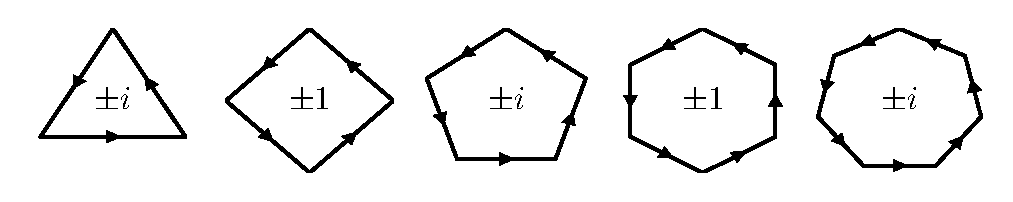
\includegraphics[width=0.86\textwidth,height=\textheight]{figure_code/amk_chapter/intro/regular_plaquettes/regular_plaquettes}
\caption[{Plaquettes in the Kitaev Model}]{The eigenvalues of a loop or plaquette operators depend on the number of bonds in its enclosing path.}
\label{fig:regular_plaquettes}
\end{figure}
}

Remarkably, all of the spin bond operators \(K_{ij}\) commute with all the Wilson loop operators \(W_p\). \[[W_p, K_{ij}] = 0\] We can prove this by considering three cases: 1. neither \(i\) nor \(j\) is part of the loop 2. one of \(i\) or \(j\) are part of the loop 3. both are part of the loop

The first case is trivial. The other two require some algebra, outlined in \cref{fig:visual_kitaev_2}.

\hypertarget{fig:visual_kitaev_2}{%
\begin{figure}
\centering
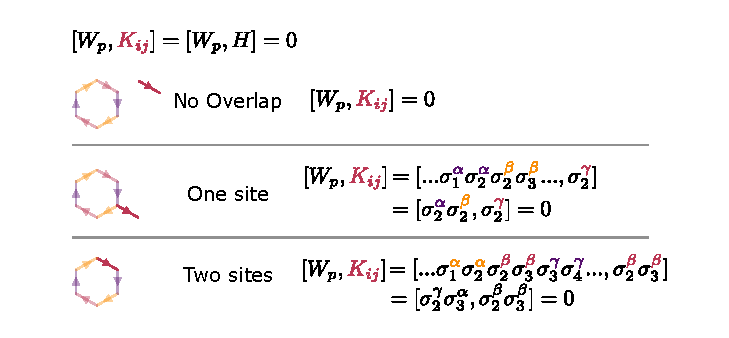
\includegraphics[width=1\textwidth,height=\textheight]{figure_code/amk_chapter/visual_kitaev_2}
\caption[{Plaquette Operators are Conserved}]{Plaquette operators are conserved.}
\label{fig:visual_kitaev_2}
\end{figure}
}

Since the Hamiltonian is a linear combination of bond operators, it commutes with the plaquette operators. This is helpful because it leads to a simultaneous eigenbasis for the Hamiltonian and the plaquette operators. We can, thus, work in \emph{or ``on''???} a basis in which the eigenvalues of the plaquette operators take on a definite value and, for all intents and purposes, act like classical degrees of freedom. These are the extensively many conserved quantities that make the model tractable.

Plaquette operators measure flux. We will find that the ground state of the model corresponds to some particular choice of flux through each plaquette. We will refer to excitations which flip the expectation value of a plaquette operator away from the ground state as \textbf{vortices}.

Thus, fixing a configuration of the vortices partitions the many-body Hilbert space into a set of `vortex sectors' labelled by that particular flux configuration \(\phi_i = \pm 1,\pm i\).

\hypertarget{from-spins-to-majorana-operators}{%
\subsubsection{From Spins to Majorana operators}\label{from-spins-to-majorana-operators}}

\hypertarget{for-a-single-spin}{%
\paragraph{For a single spin}\label{for-a-single-spin}}

Let us start by considering only one site and its \(\sigma^x, \sigma^y\) and \(\sigma^z\) operators which live in a two dimensional Hilbert space \(\mathcal{L}\).

We will introduce two fermionic modes \(f\) and \(g\) that satisfy the canonical anticommutation relations along with their number operators \(n_f = f^\dagger f, n_g = g^\dagger g\) and the total fermionic parity operator \(F_p = (2n_f - 1)(2n_g - 1)\) which can be used to divide their Fock space up into even and odd parity subspaces. These subspaces are separated by the addition or removal of one fermion.

From these two fermionic modes, we can build four Majorana operators: \[\begin{aligned}
b^x &= f + f^\dagger\\
b^y &= -i(f - f^\dagger)\\
b^z &= g + g^\dagger\\
c   &= -i(g - g^\dagger)
\end{aligned}\]

The Majoranas obey the usual commutation relations, squaring to one and anticommuting with each other. The fermions and Majorana live in a four dimensional Fock space \(\mathcal{\tilde{L}}\). We can therefore identify the two dimensional space \(\mathcal{M}\) with one of the parity subspaces of \(\mathcal{\tilde{L}}\) which will be called the \emph{physical subspace} \(\mathcal{\tilde{L}}_p\). Kitaev defines the operator \[D = b^xb^yb^zc\] which can be expanded to \[D = -(2n_f - 1)(2n_g - 1) = -F_p\] and labels the physical subspace as the space spanned by states for which \[ D|\phi\rangle = |\phi\rangle\]

We can also think of the physical subspace as whatever is left after applying the projector \[P  = \frac{1 - D}{2}\] This formulation will be useful for taking states that span the extended space \(\mathcal{\tilde{M}}\) and projecting them into the physical subspace.

So now, with the caveat that we are working in the physical subspace, we can define new Pauli operators:

\[\tilde{\sigma}^x = i b^x c,\; \tilde{\sigma}^y = i b^y c,\; \tilde{\sigma}^y = i b^y c\]

These extended space Pauli operators satisfy all the usual commutation relations. The only difference is that if we evaluate \(\sigma^x \sigma^y \sigma^z = i\), we instead get \[ \tilde{\sigma}^x\tilde{\sigma}^y\tilde{\sigma}^z = iD \]

This makes sense if we promise to confine ourselves to the physical subspace \(D = 1\).

\hypertarget{for-multiple-spins}{%
\paragraph{For multiple spins}\label{for-multiple-spins}}

This construction easily generalises to the case of multiple spins. We get a set of 4 Majoranas \(b^x_j,\; b^y_j,\;b^z_j,\; c_j\) and a \(D_j = b^x_jb^y_jb^z_jc_j\) operator for every spin. For a state to be physical, we require that \(D_j |\psi\rangle = |\psi\rangle\) for all \(j\).

From these each Pauli operator can be constructed: \[\tilde{\sigma}^\alpha_j = i b^\alpha_j c_j\]

This is where the magic happens. We can promote the spin hamiltonian from \(\mathcal{L}\) into the extended space \(\mathcal{\tilde{L}}\), safe in the knowledge that nothing changes so long as we only actually work with physical states. The Hamiltonian \[\begin{aligned}
\tilde{H} &=  - \sum_{\langle j,k\rangle_\alpha} J^{\alpha}\tilde{\sigma}_j^{\alpha}\tilde{\sigma}_k^{\alpha}\\
          &= \frac{i}{4} \sum_{\langle j,k\rangle_\alpha} 2J^{\alpha} (ib^\alpha_i b^\alpha_j) c_i c_j\\
          &=  \frac{i}{4} \sum_{\langle i,j\rangle_\alpha} 2J^{\alpha} \hat{u}_{ij} \hat{c}_i \hat{c}_j
\end{aligned}\]

We can factor out the Majorana bond operators \(\hat{u}_{ij} = i b^\alpha_i b^\alpha_j\). Note that these bond operators are not equal to the spin bond operators \(K_{ij} = \sigma^\alpha_i \sigma^\alpha_j = - \hat{u}_{ij} c_i c_j\). In what follows, we will work much more frequently with the Majorana bond operators. Therefore, when we refer to bond operators without qualification, we are referring to the Majorana variety.

Similarly to the argument with the spin bond operators \(K_{ij}\), we can quickly verify by considering three cases that the Majorana bond operators \(u_{ij}\) all commute with one another. They square to one, so have eigenvalues \(\pm 1\). They also commute with the \(c_i\) operators.

Importantly, the operators \(D_i = b^x_i b^y_i b^z_i c_i\) commute with \(K_{ij}\) and, therefore, with \(\tilde{H}\). We will show later that the action of \(D_i\) on a state is to flip the values of the three \(u_{ij}\) bonds that connect to site \(i\). Physically, this indicates that \(u_{ij}\) is a gauge field with a high degree of degeneracy.

In summary, Majorana bond operators \(u_{ij}\) are an emergent, classical, \(\mathbb{Z_2}\) gauge field!

\hypertarget{partitioning-the-hilbert-space-into-bond-sectors}{%
\subsubsection{Partitioning the Hilbert Space into Bond sectors}\label{partitioning-the-hilbert-space-into-bond-sectors}}

Similarly to the story with the plaquette operators from the spin language, we can divide the Hilbert space \(\mathcal{L}\) into sectors labelled by a set of choices \(\{\pm 1\}\) for the value of each \(u_{ij}\) operator which we denote by \(\mathcal{L}_u\). Since \(u_{ij} = -u_{ji}\), we can represent the \(u_{ij}\) graphically with an arrow that points along each bond in the direction in which \(u_{ij} = 1\).

Once confined to a particular \(\mathcal{L}_u\), we can `remove the hats' from the \(\hat{u}_{ij}\). The hamiltonian becomes a quadratic, free fermion problem \[\tilde{H_u} =  \frac{i}{4} \sum_{\langle i,j\rangle_\alpha} 2J^{\alpha} u_{ij} c_i c_j\] The ground state, \(|\psi_u\rangle\) can be found easily as will be explained in the next part. At this point, we may wonder whether the \(\mathcal{L}_u\) are confined entirely within the physical subspace \(\mathcal{L}_p\) and, indeed, we will see that they are not. However, it will be helpful to first develop the theory of the Majorana Hamiltonian further.

\hypertarget{the-majorana-hamiltonian}{%
\subsection{The Majorana Hamiltonian}\label{the-majorana-hamiltonian}}

We now have a quadratic Hamiltonian \[ \tilde{H} =  \frac{i}{4} \sum_{\langle i,j\rangle_\alpha} 2J^{\alpha} u_{ij} c_i c_j\] in which most of the Majorana degrees of freedom have paired along bonds to become a classical gauge field \(u_{ij}\). What follows is relatively standard theory for quadratic Majorana Hamiltonians \autocite{BlaizotRipka1986}.

Because of the antisymmetry of the matrix with entries \(J^{\alpha} u_{ij}\), the eigenvalues of the Hamiltonian \(\tilde{H}_u\) come in pairs \(\pm \epsilon_m\). This redundant information is a consequence of the doubling of the Hilbert space which occurred when we transformed to the Majorana representation.

If we organise the eigenmodes of \(H\) into pairs, such that \(b_m\) and \(b_m'\) have energies \(\epsilon_m\) and \(-\epsilon_m\), we can construct the transformation \(Q\) \[(c_1, c_2... c_{2N}) Q = (b_1, b_1', b_2, b_2' ... b_{N}, b_{N}')\] and put the Hamiltonian into the form \[\tilde{H}_u = \frac{i}{2} \sum_m \epsilon_m b_m b_m'\]

The determinant of \(Q\) will be useful later when we consider the projector from \(\mathcal{\tilde{L}}\) to \(\mathcal{L}\). Otherwise, the \(b_m\) are merely an intermediate step. From them, we form fermionic operators \[ f_i = \tfrac{1}{2} (b_m + ib_m')\] with their associated number operators \(n_i = f^\dagger_i f_i\). These let us write the Hamiltonian neatly as

\[ \tilde{H}_u = \sum_m \epsilon_m (n_m - \tfrac{1}{2}).\]

The ground state \(|n_m = 0\rangle\) of the many body system at fixed \(u\) is then \[E_{u,0} = -\frac{1}{2}\sum_m \epsilon_m \] We can construct any state from a particular choice of \(n_m = 0,1\).

If we only care about the value of \(E_{u,0}\), it is possible to skip forming the fermionic operators. The eigenvalues obtained directly from diagonalising \(J^{\alpha} u_{ij}\) come in \(\pm \epsilon_m\) pairs. We can take half the absolute value of the whole set to recover \(\sum_m \epsilon_m\) easily.

Takeaway: the Majorana Hamiltonian is quadratic within a Bond Sector.

\hypertarget{mapping-back-from-bond-sectors-to-the-physical-subspace}{%
\subsubsection{Mapping back from Bond Sectors to the Physical Subspace}\label{mapping-back-from-bond-sectors-to-the-physical-subspace}}

At this point, given a particular bond configuration \(u_{ij} = \pm 1\), we can construct a quadratic Hamiltonian \(\tilde{H}_u\) in the extended space and diagonalise it to find its ground state \(|\vec{u}, \vec{n} = 0\rangle\). This is not necessarily the ground state of the system as a whole, it is just the lowest energy state within the subspace \(\mathcal{L}_u\)

\textbf{However, \(|u, n_m = 0\rangle\) does not lie in the physical subspace}. As an example, consider the lowest energy state associated with \(u_{ij} = +1\). This state satisfies \[u_{ij} |\vec{u}=1, \vec{n} = 0\rangle = |\vec{u}=1, \vec{n} = 0\rangle\] for all bonds \(i,j\).

If we act on it, this state with one of the gauge operators \(D_j = b_j^x b_j^y b_j^z c_j\), we see that \(D_j\) flips the value of the three bonds \(u_{ij}\) that surround site \(k\):

\[ |u'\rangle = D_j |u=1, n_m = 0\rangle\]

\[ \begin{aligned}
\langle u'|u_{ij}|u'\rangle &=  \langle u| b_j^x b_j^y b_j^z c_j \;ib^x_i b^x_j\; b_j^x b_j^y b_j^z c_j|u\rangle\\
&= -1
\end{aligned}\]

Since \(D_j\) commutes with the Hamiltonian in the extended space \(\tilde{H}\), the fact that \(D_j\) flips the value of bond operators indicates that there is a gauge degeneracy between the ground state of \(\tilde{H}_u\) and the set of \(\tilde{H}_{u'}\) related to it by gauge transformations \(D_j\). Thus, we can flip any three bonds around a vertex and the physics will stay the same.

We can turn this into a symmetrisation procedure by taking a superposition of every possible gauge transformation. Every possible gauge transformation is just every possible subset of \({D_0, D_1 ... D_n}\) which can be neatly expressed as \[|\phi_w\rangle = \prod_i \left( \frac{1 + D_i}{2}\right) |\tilde{\phi}_u\rangle\] This is convenient because the quantity \(\frac{1 + D_i}{2}\) is also the local projector onto the physical subspace. Here \(|\phi_w\rangle\) is a gauge invariant state that lives in \(\mathcal{L}_p\) which has been constructed from a set of states in different \(\mathcal{L}_u\).

This gauge degeneracy leads us to the next topic of discussion, namely how to construct a set of gauge invariant quantities out of the \(u_{ij}\), these will turn out to just be the plaquette operators.

Takeaway: The Bond Sectors overlap with the physical subspace but are not contained within it.

\hypertarget{open-boundary-conditions}{%
\subsubsection{Open boundary conditions}\label{open-boundary-conditions}}

Care must be taken when defining open boundary conditions. Simply removing bonds from the lattice leaves behind unpaired \(b^\alpha\) operators that must be paired in some way to arrive at fermionic modes. To fix a pairing, we always start from a lattice defined on the torus and generate a lattice with open boundary conditions by defining the bond coupling \(J^{\alpha}_{ij} = 0\) for sites joined by bonds \((i,j)\) that we want to remove. This creates fermionic zero modes \(u_{ij}\) associated with these cut bonds which we set to 1 when calculating the projector.

Alternatively, since all the fermionic zero modes are degenerate anyway, an arbitrary pairing of the unpaired \(b^\alpha\) operators could be performed. \textless/i,j\textgreater\textless/i,j\textgreater{}
